% ============================================
% Chapter 5: Model Training and Evaluation
% ============================================
% Rewritten — June 2026
% Based on Khadija's ML pipeline work, retrained models

\chapter{Model Training and Evaluation}

\section{Introduction}

With the dataset cleaned, standardized, and balanced (Chapter~4), this chapter addresses the core question of the detection module: \textbf{can machine learning reliably distinguish port scan traffic from benign traffic?}

To answer this, we train and evaluate three complementary models:

\begin{itemize}
    \item \textbf{Random Forest} --- a robust supervised classifier based on ensemble learning. Chosen as the primary detection model because it handles high-dimensional tabular data well and provides feature importance scores.
    \item \textbf{XGBoost} --- a state-of-the-art gradient boosting algorithm. Included as a comparison point to verify that the simpler Random Forest is not being outperformed by a more sophisticated approach.
    \item \textbf{Isolation Forest} --- an unsupervised anomaly detector. Included to test whether port scans can be detected as statistical anomalies without needing labeled training data. This is particularly relevant for detecting \textit{low-and-slow} (stealthy) scans that might evade supervised models trained on aggressive scan signatures.
\end{itemize}

\section{Model Descriptions}

Before presenting the results, it is important to understand how each model works and why it was chosen for this specific problem.

\subsection{Random Forest}

\textbf{How it works:} Random Forest builds an ensemble of $n$ decision trees (we use $n=100$), each trained on a random subset of the data and a random subset of the features. The final prediction is the \textbf{majority vote} of all 100 trees. This process is called \textit{bagging} (\textit{Bootstrap Aggregating}) and it makes the model extremely resistant to overfitting.

\textbf{Why for port scan detection:}
\begin{itemize}
    \item Tabular network data with 11 features is exactly the type of problem where Random Forest excels.
    \item The model provides \textbf{feature importance} scores, telling us which features (SYN flags? flow duration? destination ports?) are most useful for detection --- valuable for understanding what makes a port scan recognizable.
    \item It requires minimal hyperparameter tuning; the default parameters already produce excellent results on this type of data.
\end{itemize}

\begin{lstlisting}[caption={Random Forest training}]
from sklearn.ensemble import RandomForestClassifier

rf = RandomForestClassifier(
    n_estimators=100,    # 100 trees in the forest
    random_state=42      # Reproducibility
)
rf.fit(X_train_res, y_train_res)
joblib.dump(rf, "../models/saved/rf_model.pkl")
\end{lstlisting}

\subsection{XGBoost (eXtreme Gradient Boosting)}

\textbf{How it works:} Unlike Random Forest, which builds trees in parallel, XGBoost builds trees \textbf{sequentially}. Each new tree is trained to correct the errors of the previous trees, using gradient descent to minimize a loss function. The model also includes $L_1$ and $L_2$ regularization to prevent overfitting.

\textbf{Why for port scan detection:}
\begin{itemize}
    \item XGBoost is considered state-of-the-art for tabular data and consistently wins Kaggle competitions.
    \item Its sequential training approach can capture subtle patterns that parallel ensemble methods might miss.
    \item Including XGBoost as a comparison point validates that Random Forest's performance is not due to model simplicity --- it confirms the features themselves (not the model choice) drive the high detection rate.
\end{itemize}

\begin{lstlisting}[caption={XGBoost training}]
from xgboost import XGBClassifier

xgb = XGBClassifier(
    n_estimators=100,
    learning_rate=0.1,   # Step size for gradient descent
    max_depth=6,         # Maximum tree depth (prevents overfitting)
    random_state=42,
    eval_metric="logloss"
)
xgb.fit(X_train_res, y_train_res)
joblib.dump(xgb, "../models/saved/xgb_model.pkl")
\end{lstlisting}

\subsection{Isolation Forest}

\textbf{How it works:} Isolation Forest is fundamentally different from the two supervised models. It is \textbf{unsupervised} --- it does not learn to distinguish PortScan from BENIGN because it never sees labels during training. Instead, it learns what "normal" data looks like and flags anything anomalous. The core idea: anomalies are \textit{few and different}, meaning they can be isolated from the rest of the data with fewer random splits in a tree structure. The fewer splits needed to isolate a point, the more likely it is an anomaly.

\textbf{Why for port scan detection:}
\begin{itemize}
    \item In a real network, attackers often use \textit{low-and-slow} techniques --- sending probes slowly over hours to avoid detection. These attacks may not match the aggressive scan patterns in the training data.
    \item An unsupervised model can, in theory, flag \textbf{any} unusual behavior as suspicious, even if it has never seen that exact attack pattern before.
    \item This provides a complementary detection layer: supervised models catch known patterns, unsupervised models catch the unknown.
\end{itemize}

\begin{lstlisting}[caption={Isolation Forest training (unsupervised)}]
from sklearn.ensemble import IsolationForest

iso = IsolationForest(
    contamination='auto',  # Let the model estimate the anomaly ratio
    random_state=42
)
iso.fit(X_train_scaled)    # Trained WITHOUT labels
joblib.dump(iso, "../models/saved/isolation_forest.pkl")
\end{lstlisting}

\section{Training Process}

\subsection{Cross-Validation}

To ensure the results are statistically reliable and not dependent on a particular random split of the data, we use \textbf{10-fold Stratified Cross-Validation} on the supervised models.

\textbf{How it works:} The training data is divided into 10 equal parts (\textit{folds}). In each of 10 iterations, 9 folds are used for training and the 1 remaining fold is used for validation. The process repeats until every fold has served as the validation set once. The final score is the average of all 10 iterations.

\begin{figure}[H]
\centering
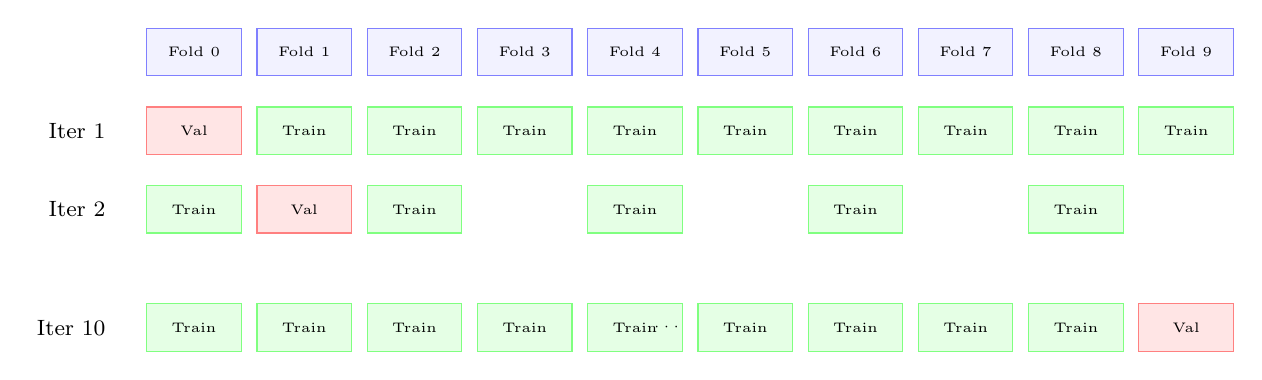
\begin{tikzpicture}[
    node distance=0.8cm,
    fold/.style={rectangle, draw=blue!50, fill=blue!5, minimum width=1.2cm, minimum height=0.6cm, font=\tiny},
    train/.style={rectangle, draw=green!50, fill=green!10, minimum width=1.2cm, minimum height=0.6cm, font=\tiny},
    val/.style={rectangle, draw=red!50, fill=red!10, minimum width=1.2cm, minimum height=0.6cm, font=\tiny},
]
    % Fold labels
    \foreach \i in {0,...,9} {
        \node[fold] at (\i*1.4, 0) {Fold \i};
    }
    % Iteration 1
    \foreach \i in {1,...,9} { \node[train] at (\i*1.4, -1) {Train}; }
    \node[val] at (0, -1) {Val};
    % Iteration 2
    \foreach \i in {0,2,...,9} { \node[train] at (\i*1.4, -2) {Train}; }
    \node[val] at (1.4, -2) {Val};
    % Iteration 10
    \foreach \i in {0,...,8} { \node[train] at (\i*1.4, -3.5) {Train}; }
    \node[val] at (12.6, -3.5) {Val};
    \node[font=\tiny] at (6, -3.5) {$\cdots$};
    % Labels
    \node[font=\footnotesize, anchor=east] at (-1, -1) {Iter 1};
    \node[font=\footnotesize, anchor=east] at (-1, -2) {Iter 2};
    \node[font=\footnotesize, anchor=east] at (-1, -3.5) {Iter 10};
\end{tikzpicture}
\caption{10-fold cross-validation: each fold serves as the validation set exactly once. The final score is the average of all 10 iterations, providing a robust estimate of model performance.}
\label{fig:cv}
\end{figure}

\begin{table}[H]
\centering
\caption{Stratified cross-validation results (10 folds, F1-Score)}
\label{tab:cv_results}
\begin{tabular}{lcc}
\toprule
\textbf{Model} & \textbf{Mean F1} & \textbf{Std Dev ($\pm 2\sigma$)} \\
\midrule
Random Forest & 0.9993 & $\pm$ 0.0003 \\
XGBoost & 0.9994 & $\pm$ 0.0003 \\
\bottomrule
\end{tabular}
\end{table}

The extremely low standard deviation ($\pm 0.0003$) confirms that both models perform consistently across all folds --- there is no overfitting to a particular subset of the data. Note that Isolation Forest, being unsupervised, cannot be evaluated via cross-validation on F1 score (it never sees labels during training).

\section{Understanding the Evaluation Metrics}

Before presenting the numerical results, it is important to define what each metric actually means. In network intrusion detection, different metrics serve different purposes:

\begin{itemize}
    \item \textbf{Accuracy} — The percentage of all predictions that were correct: $\frac{TP + TN}{TP + TN + FP + FN}$. This is the simplest metric but can be misleading if the classes are imbalanced.

    \item \textbf{Precision} — Of all the flows the model flagged as attacks, what percentage actually were attacks: $\frac{TP}{TP + FP}$. \textbf{High precision means few false alarms.}

    \item \textbf{Recall} — Of all the actual attack flows in the data, what percentage did the model catch: $\frac{TP}{TP + FN}$. \textbf{High recall means few missed attacks.}

    \item \textbf{F1-Score} — The harmonic mean of precision and recall: $2 \times \frac{P \times R}{P + R}$. This is the best single-number summary when both false alarms and missed attacks matter.

    \item \textbf{False Positive Rate (FPR)} — What percentage of benign flows were incorrectly flagged as attacks: $\frac{FP}{FP + TN}$. \textbf{Low FPR means the system does not cry wolf.}

    \item \textbf{AUC-ROC} — The area under the ROC curve. A value of 0.5 means the model is no better than random guessing; 1.0 means perfect discrimination at every threshold.
\end{itemize}

\begin{table}[H]
\centering
\caption{Confusion matrix terminology}
\label{tab:cm_terms}
\begin{tabular}{llp{7cm}}
\toprule
\textbf{Term} & \textbf{Meaning} & \textbf{In our context} \\
\midrule
TP (True Positive) & Correctly classified as attack & Port scan correctly detected as port scan \\
TN (True Negative) & Correctly classified as benign & Normal traffic correctly identified as normal \\
FP (False Positive) & Benign incorrectly classified as attack & Normal traffic falsely triggers an alert \\
FN (False Negative) & Attack missed (classified as benign) & Port scan goes undetected \\
\bottomrule
\end{tabular}
\end{table}

\noindent\textbf{Where:} $TP$ = True Positive, $TN$ = True Negative, $FP$ = False Positive, $FN$ = False Negative.

\section{Results and Analysis}

\subsection{Supervised Models: Random Forest and XGBoost}

Both supervised models deliver exceptional performance on the CICIDS2017 test set:

\begin{table}[H]
\centering
\caption{Performance comparison of all three models on the CICIDS2017 test set (57,294 samples)}
\label{tab:results}
\begin{tabular}{lcccccc}
\toprule
\textbf{Model} & \textbf{Accuracy} & \textbf{Precision} & \textbf{Recall} & \textbf{F1-Score} & \textbf{AUC-ROC} & \textbf{FPR} \\
\midrule
Random Forest & 99.911\% & 99.909\% & 99.931\% & 99.920\% & 0.9997 & 0.114\% \\
XGBoost & 99.914\% & 99.909\% & 99.937\% & 99.923\% & 0.9999 & 0.114\% \\
Isolation Forest & 24.627\% & 14.184\% & 7.101\% & 9.464\% & --- & 53.532\% \\
\bottomrule
\end{tabular}
\end{table}

\textbf{What these numbers mean in practice:}
\begin{itemize}
    \item Out of 57,294 test flows (31,786 attacks + 25,508 benign), Random Forest makes only 51 mistakes total: 29 false positives (benign flagged as attack) and 22 false negatives (attacks missed).
    \item XGBoost makes 49 mistakes: 29 false positives and 20 false negatives.
    \item The 0.114\% FPR means that out of 1,000 benign flows, the system incorrectly raises an alert for approximately 1 --- an acceptable rate for a production environment.
\end{itemize}

\begin{figure}[H]
\centering
\begin{subfigure}[b]{0.48\textwidth}
\includegraphics[width=\textwidth]{confusion_matrix_random_forest.png}\caption{Random Forest}\end{subfigure}\hfill
\begin{subfigure}[b]{0.48\textwidth}
\includegraphics[width=\textwidth]{confusion_matrix_xgboost.png}\caption{XGBoost}\end{subfigure}
\caption{Confusion matrices for the supervised models. Both models make very few errors: the vast majority of predictions fall on the diagonal (correct classifications).}
\label{fig:confusion_matrices}
\end{figure}

\begin{figure}[H]
\centering
\begin{subfigure}[b]{0.48\textwidth}
\includegraphics[width=\textwidth]{roc_random_forest.png}\caption{Random Forest}\end{subfigure}\hfill
\begin{subfigure}[b]{0.48\textwidth}
\includegraphics[width=\textwidth]{roc_xgboost.png}\caption{XGBoost}\end{subfigure}
\caption{ROC curves for the supervised models. Both achieve AUC $> 0.999$, indicating near-perfect discrimination between BENIGN and PortScan traffic at every possible classification threshold.}
\label{fig:roc_curves}
\end{figure}

\subsection{Success Criteria Verification}

The project's final plan defines three quantitative thresholds. Both supervised models not only meet these criteria --- they vastly exceed them:

\begin{table}[H]
\centering
\caption{Verification of project success criteria}
\label{tab:success}
\begin{tabular}{lccccc}
\toprule
\textbf{Criterion} & \textbf{Threshold} & \textbf{RF} & \textbf{Status} & \textbf{XGBoost} & \textbf{Status} \\
\midrule
F1-Score & $\geq$ 88\% & 99.920\% & \textbf{PASS} & 99.923\% & \textbf{PASS} \\
Accuracy & $\geq$ 90\% & 99.911\% & \textbf{PASS} & 99.914\% & \textbf{PASS} \\
FPR & $<$ 6\% & 0.114\% & \textbf{PASS} & 0.114\% & \textbf{PASS} \\
\bottomrule
\end{tabular}
\end{table}

\subsection{Analysis of Isolation Forest's Failure}

Isolation Forest performs very poorly on the CICIDS2017 dataset: with an F1-Score of only 9.46\% and an FPR of 53.53\%, it is essentially unusable for this dataset. However, this result is expected and does not indicate a flaw in the choice of algorithm --- it reveals a fundamental property of the dataset.

\subsubsection{The Majority Anomaly Paradox}

Isolation Forest is designed to detect anomalies -- data points that are \textit{few and different} from the rest of the dataset. The algorithm works by randomly partitioning the feature space: points that can be isolated with few partitions (short average path length in the isolation tree) are considered anomalies.

This assumption works well when anomalies represent a small fraction of the data (typically $<$ 5\%). However, in our CICIDS2017 dataset, the PortScan class constitutes \textbf{55.48\%} of the data -- it is the \textbf{majority} class, not a minority:

\begin{figure}[H]
\centering
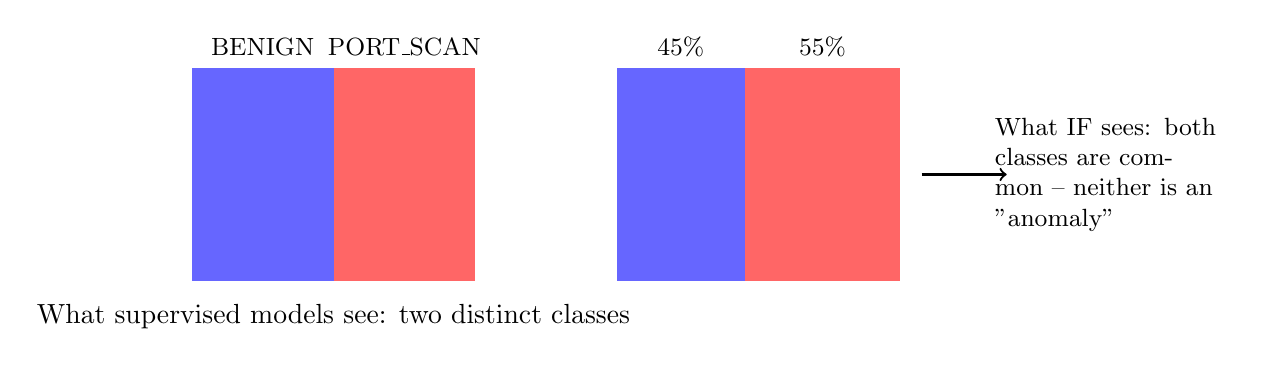
\begin{tikzpicture}[scale=0.9]
    % Bar for RF/XGB
    \fill[blue!60] (0,0) rectangle (2, 3);
    \fill[red!60] (2,0) rectangle (4, 3);
    \node[font=\small] at (1, 3.3) {BENIGN};
    \node[font=\small] at (3, 3.3) {PORT\_SCAN};
    \node[font=\normalsize] at (2, -0.5) {What supervised models see: two distinct classes};

    % Bar for IF
    \fill[blue!60] (6,0) rectangle (7.8, 3);
    \fill[red!60] (7.8,0) rectangle (10, 3);
    \node[font=\small] at (6.9, 3.3) {45\%};
    \node[font=\small] at (8.9, 3.3) {55\%};
    \draw[->, thick] (10.3, 1.5) -- (11.5, 1.5);
    \node[font=\small, text width=3cm] at (13, 1.5) {What IF sees: both classes are common -- neither is an "anomaly"};
\end{tikzpicture}
\caption{The majority anomaly paradox: when the "anomaly" (PortScan) is actually the majority class, Isolation Forest cannot isolate it as being \textit{few and different}.}
\label{fig:majority_paradox}
\end{figure}

Because the algorithm is trained on the complete dataset (BENIGN + PortScan), it sees both classes as \textit{normal} -- neither is anomalous enough to be separated from the other. The result is a model that essentially guesses at random, with a heavy bias towards the majority class.

\subsubsection{Why We Still Keep Isolation Forest}

Despite its poor performance on CICIDS2017, Isolation Forest remains part of the AEGIS architecture for two reasons:

\begin{enumerate}
    \item \textbf{Correct deployment strategy:} In production, Isolation Forest should be trained exclusively on verified \textbf{BENIGN} traffic to establish a clean baseline of normal network behavior. When trained this way (semi-supervised), it can effectively detect anything deviating from normal -- including never-before-seen attack patterns.

    \item \textbf{Complementary detection:} Supervised models (RF, XGBoost) detect \textit{known} attack patterns they were trained on. Isolation Forest, trained on benign-only data, can detect \textit{unknown} patterns -- low-and-slow scans, custom scanners, zero-day reconnaissance techniques. The two approaches complement each other.
\end{enumerate}

\begin{figure}[H]
\centering

\includegraphics[width=0.5\textwidth]{confusion_matrix_isolation_forest.png}
\caption{Confusion matrix for Isolation Forest on CICIDS2017. The high number of false positives (13,655 benign flows flagged as attacks) and false negatives (29,529 attacks missed) confirms that the unsupervised approach fails when trained on the full imbalanced dataset.}
\label{fig:iso_cm}
\end{figure}

\section{Conclusion}

This chapter presented the training and evaluation of the three models that form the core of the AEGIS detection pipeline. The results are clear:

\begin{enumerate}
    \item \textbf{Supervised models dominate on this problem.} Random Forest and XGBoost achieve F1-Scores exceeding 99.92\%, with FPRs below 0.12\%. Both models far exceed the project's success criteria (F1 $\geq$ 88\%, Accuracy $\geq$ 90\%, FPR $<$ 6\%). The 10-fold cross-validation confirms these results are stable and reproducible.

    \item \textbf{Isolation Forest fails on CICIDS2017 for a predictable reason.} The majority anomaly paradox -- PortScan being 55\% of the data -- prevents the unsupervised algorithm from usefully separating the classes. This is not a flaw in the algorithm but a mismatch between the training strategy (full dataset, unsupervised) and what the algorithm requires (benign-only, semi-supervised). In a production environment with benign-only training, the model would regain its relevance.

    \item \textbf{The feature set is sufficient.} With only 11 features, both supervised models achieve near-perfect classification. This validates the feature selection done in Chapter~4 and suggests that the 9 CICIDS2017 features carry strong discriminative signal for port scan detection. The 2 placeholder features (shadow node interaction, MTD port delta) will provide additional signal when integrated with the real-time defense subsystems (Chapter~7).
\end{enumerate}

The trained models are saved in \texttt{models/saved/} and are ready for integration with the capture layer (Chapter~6), the defense subsystem (Chapter~7), and the dashboard (Chapter~8).
